% !TeX root = ../../main.tex
% ------------------------------------------------------------------
%  4.2 Arquitectura física: título e introducción.
%
%  Este archivo lo incluye contenido.tex; las rutas de las figuras se
%  escriben desde la carpeta del subdocumento, no desde la de main.tex.
%
%  El índice obligatorio numera esta parte como 4.2.
% ------------------------------------------------------------------

% Las aclaraciones (sección 5) piden tablas sin palabras cortadas en
% columnas angostas. Esto lo activa desde aquí hasta el final del
% subdocumento, T-11 incluido.
\ifdefined\LFXcuerpotablaorig\else
  \let\LFXcuerpotablaorig\LFXcuerpotabla
  \renewcommand{\LFXcuerpotabla}{%
    \LFXcuerpotablaorig\hyphenpenalty=10000\exhyphenpenalty=10000\relax}
\fi

\section{Arquitectura física}
\markboth{Arquitectura física}{}
\phantomsection\label{fuente-02-0-arquitectura-fisica}
\label{cap:4-2-arquitectura-fisica}

La arquitectura física fija emplazamiento, servicios de nube, conexiones, contingencias y capacidad.

El despliegue híbrido del Artículo 16\textdegree{} (Bases Administrativas, art. 16, p. 11) combina AWS sa-east-1 (São Paulo) con recuperación en us-east-1 (Norte de Virginia) y continuidad local. Cubre los CD de Talca y Concepción, los cross-docking de Curicó, Chillán y Los Ángeles, la casa matriz, el terreno y 14.200 puntos de entrega. Cinco instalaciones alojan cómputo; la casa matriz, contigua al CD Talca, usa la nube. La séptima instalación prevista a tres años se incorpora por parametrización, sin desarrollo ni crecimiento de servidores en Talca. El diseño sigue dos principios:

\begin{itemize}
  \item \textbf{Carga principal en nube:} el núcleo transaccional de preventa, reparto y canal moderno, la analítica, la integración y el almacenamiento consolidado se ejecutan en AWS sa-east-1, con escalado elástico para el peak de septiembre.
  \item \textbf{Autonomía total de la operación de bodega:} la preparación, el despacho, la recepción y el conteo corren contra los servidores del centro de distribución sin depender de Internet. La guía de despacho se preemite al cerrar la carga nocturna, en Talca desde su cola local y en los demás sitios por sus caminos de enlace. Si cambia la carga entre las 05:30 y las 07:00, se invalida la guía y el ERP de Talca emite otra por cualquiera de sus tres caminos, a los que Concepción y los cross-docking llegan por los suyos. Si no hay camino hasta el ERP, el camión sale solo con la carga amparada por su guía vigente y el ajuste pasa a la ruta siguiente. Una guía ya anulada no se reutiliza: esa salida espera un documento válido.
\end{itemize}

La Figura~\ref{fig:vista-general} sitúa los componentes y conexiones del despliegue híbrido.

\begin{landscape}
\begin{figure}[p]
  \centering
  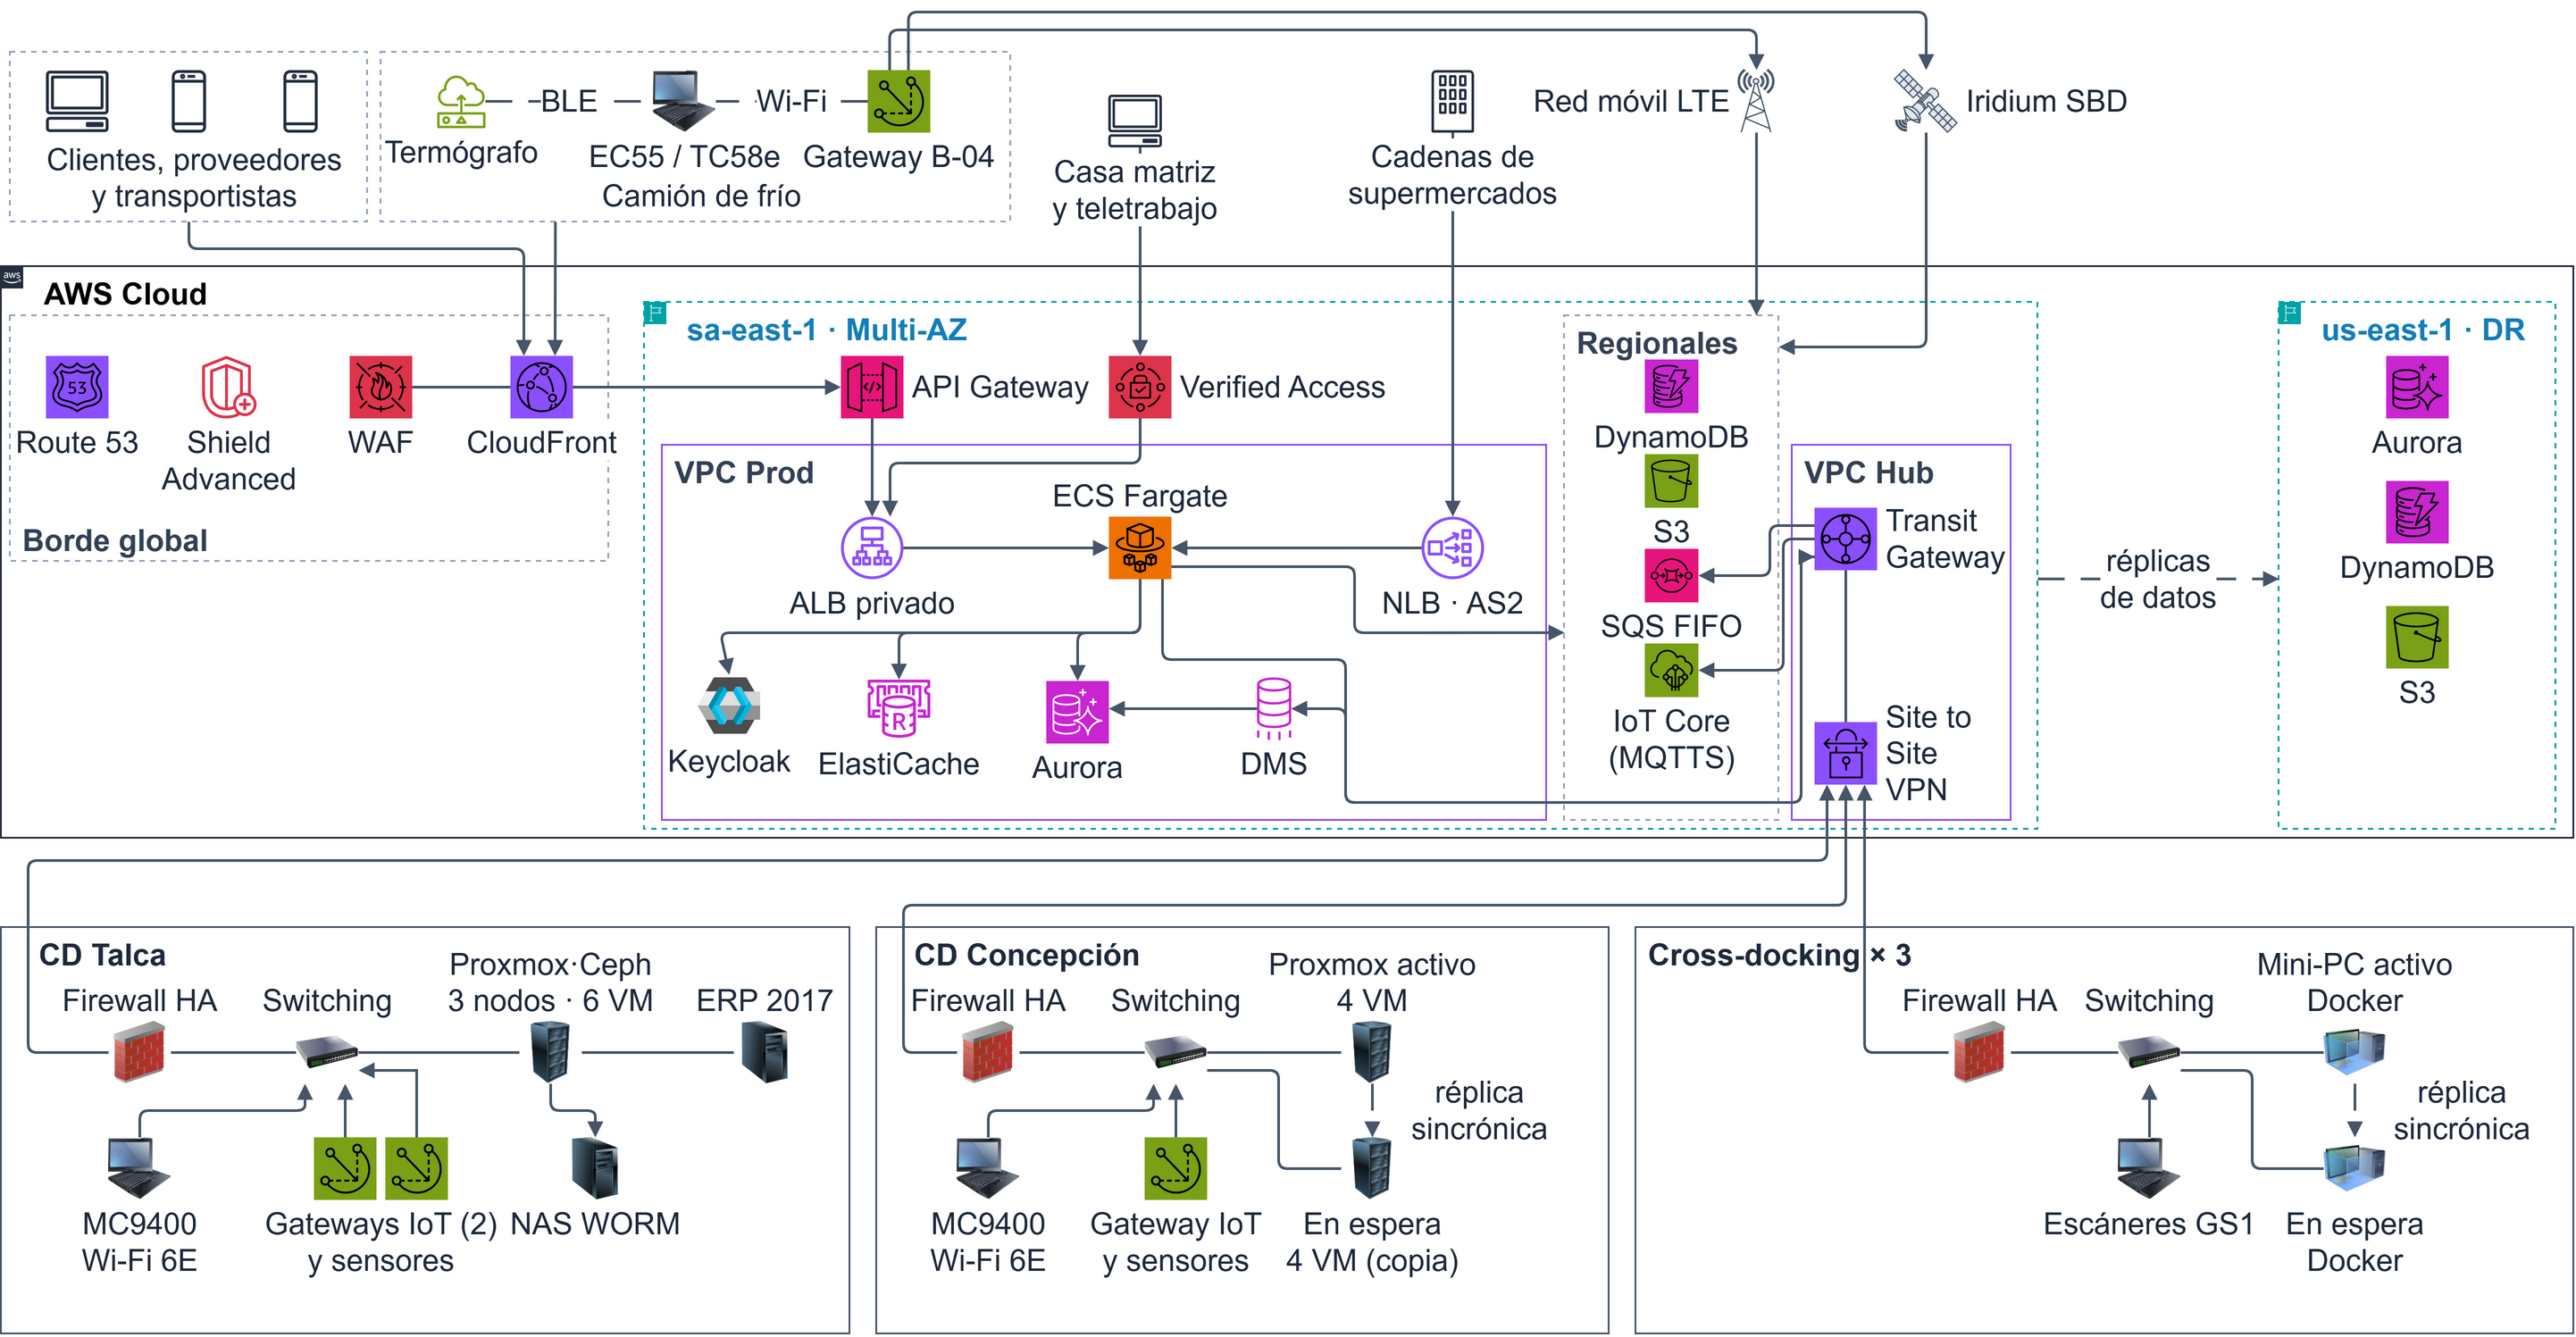
\includegraphics[width=\linewidth,height=0.9\textheight,keepaspectratio]{figuras/fisica/Arquitectura_Fisica_General.png}
  \caption{Vista general de la arquitectura física híbrida}
  \label{fig:vista-general}
  {\fontsize{9pt}{11pt}\selectfont\raggedright Fuente: elaboración propia a partir de los requisitos de arquitectura híbrida de las Bases Técnicas Transversales (sección 3) y la conectividad de las Bases Técnicas del caso (sección 6).\par}
\end{figure}
\end{landscape}

La franja superior reúne portales, terminales TC58e, casa matriz, teletrabajo y cadenas. Portales y terminales entran por CloudFront y API Gateway; oficinas, por Verified Access; AS2, por una distribución CloudFront propia hacia su balanceador interno (sección~\ref{sec:conexiones}). En el camión, el TC58e lee el termógrafo por Bluetooth y realiza la segunda evaluación térmica; el gateway Greengrass B-04 es el evaluador principal (Figura~\ref{fig:emplazamiento-dominios}).

La franja central muestra la VPC de producción en sa-east-1, sus servicios regionales y la VPC Hub con Transit Gateway y VPN. DMS lleva VM-02 de Talca a un esquema de lectura de Aurora; IoT Core recibe la telemetría por MQTTS. Aurora, DynamoDB y S3 replican a us-east-1. La Figura~\ref{fig:nube} de la sección~\ref{sec:servicios-nube} detalla zonas, seguridad, operación y capacidad reducida de recuperación.

La franja inferior reúne los cinco sitios, cada uno con firewalls en par, switching y VPN propia. Talca aloja tres nodos Proxmox/Ceph, seis VM, el ERP de 2017 trasladado y NAS WORM (Figura~\ref{fig:cd-talca}, sección~\ref{sec:d-especificaciones-del-sitio-principal-on-}). Concepción tiene dos servidores activo/espera y cuatro VM; cada cross-docking, dos mini-PC Docker (figuras~\ref{fig:cd-concepcion} y~\ref{fig:crossdocking}, sección~\ref{sec:emplazamiento}). Los MC9400 de los CD usan Wi-Fi 6E y sus cámaras cuentan con tres gateways IoT: dos en Talca y uno en Concepción. Los terminales de cross-docking acceden al mini-PC activo.

Cada bodega confirma contra su WMS. Talca replica por DMS; los demás sitios publican eventos por SQS FIFO. Durante el corte, bases y brokers locales retienen la operación y sincronizan al reconectar. La nube concentra servicios comunes y recuperación de Talca.

El detalle se organiza en \ref{sec:implementos} (equipamiento y software; especificaciones en el Formulario T-11, archivo propio), \ref{sec:emplazamiento} (ubicación conforme al Artículo 16.2, Bases Administrativas, p. 11), \ref{sec:servicios-nube} (servicios contratados), \ref{sec:despliegue} (entrega y continuidad), \ref{sec:conexiones} (conexiones y fallas) y \ref{sec:dimensionamiento} (capacidad).

Las especificaciones del data center primario y del secundario se desarrollan en el apartado~\ref{cap:4-3-data-center}, a continuación de este.

\label{fuente-02-0-arquitectura-fisica-fin}
